\begin{frame}[t]{Wheatstone Bridge}

    Die Wheatstone Bridge ist eine einfache Schaltung um einen Wiederstand zu messen. Die Schaltung gilt als abgeglichen, wenn an $V_{AB}$ keine Spannng anliegt.

    Die theoretische Herleitung ist nicht ganz trivial (später mehr) daher möchten wir an dieser Stelle die Realität und den Aufwand eines praktischen Aufbaus mit der Flexibilität einer Simulation gegenüberstellen.


    \begin{figure}
        \scalebox{0.6}{
      \centering
      \begin{circuitikz}
        \ctikzset{bipoles/thickness=1}
        \ctikzset{bipoles/length=.6cm}
        \draw
        (0,0) to [short, *-] (4,0)
        (0,0) to [V, l_=$V_{1}$] (0,-4)
        (2,0) to (2,-0.5)
        (4,0) to (4,-0.5)
        (2,-0.5) to [R, l_=$R_{1}$] (2,-1.5)
        (2,-2.5) to [R, l_=$R_{2}$] (2,-3.5)
        (2,-1.5) to (2,-2.5)
        (2,-2) to [short,*-o] (2.25,-2) node[right]{$V_{a}$}
        (4,-1.5) to (4,-2.5)
        (4,-2) to [short,*-o] (4.25,-2) node[right]{$V_{b}$}
        (4,-0.5) to [R, l_=$R_{3}$] (4,-1.5)
        (4,-2.5) to [R, l_=$R_{4}$] (4,-3.5)
        (2,-3.5) to (2,-4)
        (4,-3.5) to (4,-4)
        (0,-4) node[ground]{}
        (2,-4) node[ground]{}
        (4,-4) node[ground]{}
        ;
        \end{circuitikz}
        }
    \end{figure}

\end{frame}

\begin{frame}[t]{Experiment}

Wir werden jetzt den folgenden Aufbau "live" analysieren. Beachtet, dass die Schaltung komplexer ist als in dem einleitenden schematischen Aufbau - wie immer.

\begin{spacing}{0.9} \begin{tiny}
    \begin{minipage}{\textwidth}
      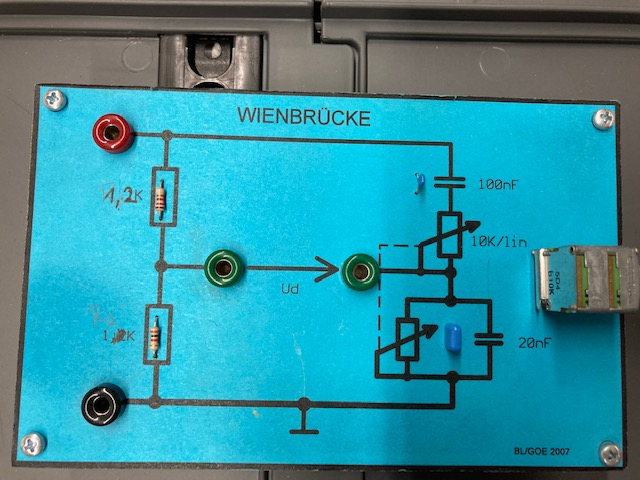
\includegraphics[width=0.5\linewidth]{pictures/wheatstone_bridge.jpg}
    \end{minipage}
\end{tiny} \end{spacing}

\textbf{Leitet aus der gemessenen Spannung den Wiederstandswert her.}

\end{frame}
